\documentclass[11pt,a4paper,twoside]{report}

%--------------------------------------------------
% global definitions to be used in the front page
%--------------------------------------------------
\providecommand{\coursename}{Progetto di Ingegneria Informatica}
\providecommand{\documentsubtitle}{Documentazione}
\providecommand{\annoacc}{2011-2012}
\providecommand{\principaladviser}{Prof. Andrea Bonarini}
\providecommand{\firstauthor}{Marcello Pogliani}
\providecommand{\firstauthorid}{742961}
\providecommand{\secondauthor}{Davide Tateo}
\providecommand{\secondauthorid}{743013}
\title{RoboTower}
\author{\firstauthor, \secondauthor}

\usepackage[margin=3cm]{geometry} % margins set here are for the TITLE page...

\usepackage[utf8]{inputenc}
\usepackage[italian]{babel}
%\usepackage{fancyhdr}
\usepackage{tikz}
\usetikzlibrary{arrows,positioning, decorations.text}

\usepackage{graphicx}
\usepackage{booktabs}
\usepackage{listings}
\lstset{columns=fullflexible}

\usepackage[T1]{fontenc}
\usepackage{palatino}
\usepackage{mathpazo} % font per caratteri matmatici simile a palatino
%\usepackage[scaled]{beramono}
\lstset{basicstyle=\ttfamily}

\usepackage[pdfauthor={\firstauthor, \secondauthor}, pdftitle={RoboTower}, colorlinks, linkcolor=black, urlcolor=black]{hyperref}

\usepackage{amsmath}
\usepackage{amsthm}
\newtheoremstyle{note} % name
	{\topsep} 	% Space above
	{\topsep} 	% Space below
	{\small}		% Body font
	{}		% Indent amount
	{\small\bfseries}% Theorem head font
	{:}		% Punctuation after theorem head
	{.5em}	% Space after theorem head
	{}		% Theorem head spec (can be left empty, meaning ‘normal’)
\theoremstyle{note}
\newtheorem*{nota}{Nota}	
%
\usepackage{settings/frontesp}

\usepackage{fancyhdr}
%% Cambia il carattere delle didascalie delle figure %%
\usepackage[font=small,format=plain,labelfont=bf,up,textfont=it,up]{caption}

\begin{document}

\titlep
\newgeometry{top=4cm,bottom=4cm,right=4cm,left=4cm}
%% STILE DELLE INTESTAZIONI %%
\usepackage{fancyhdr}
\pagestyle{fancy}
\renewcommand{\chaptermark}[1]{\markboth{#1}{}} % aggiungi \thechapter.\ per anche il numero capitolo
%\renewcommand{\sectionmark}[1]{\markright{#1}} % titoli di sezione
\fancyhf{}
\fancyhead[RE,RO]{\small\thepage}
\fancyhead[LE,LO]{\small\em\leftmark} % \leftmark = 2.TitoloCapitolo, \rightmark = TitoloSezione
%\fancyhead[LO]{\small\em\rightmark}  % LO = Left Odd, RO = Right Odd, LE = Left Even, RE = Right Even
\fancypagestyle{plain}{ % titolo di sezione e simili
	\fancyhf{} % remove everything
	\renewcommand{\headrulewidth}{0pt} % remove lines as well
	\renewcommand{\footrulewidth}{0pt}
}

%% Cambia il carattere dei titoli di sezione %%
\usepackage{titlesec}
\titleformat{\section}{\Large\bfseries\sffamily}{\thesection}{1em}{}

%% Stile dei titoli di capitolo %%
\makeatletter
\def\thickhrulefill{\leavevmode \leaders \hrule height 0.7ex \hfill \kern \z@}
\def\@makechapterhead#1{%
  \vspace*{10\p@}%
  {\parindent \z@ \centering \reset@font
        %\thickhrulefill
        \par\nobreak \vspace{3\p@}
        {\huge \bfseries \sffamily \strut \thechapter.\ #1}\par\nobreak
        \interlinepenalty\@M
        \hrule
        \vspace*{10\p@}%
    \vskip 30\p@
  }}

\def\@makeschapterhead#1{%
  \vspace*{10\p@}%
  \vspace*{10\p@}%
  {\parindent \z@ \centering \reset@font
        %\thickhrulefill
        \par\nobreak \vspace{3\p@}
        {\huge \bfseries \sffamily \strut #1}\par\nobreak
        \interlinepenalty\@M
        \hrule
        \vspace*{10\p@}%
    \vskip 30\p@
  }}


% \pagenumbering{roman}
\tableofcontents
\cleardoublepage

% \pagenumbering{arabic}
% \setcounter{1}
%\pagestyle{fancy}



% --------------------------------------------------------------------------------------------------------------------
% Capitoli
\chapter{Introduzione}
%\markboth{Introduzione}{Introduzione}
\label{cap:introduzione}

Il presente lavoro si pone come obiettivo il progetto e l'implementazione di un gioco di tipo ``HI-CoRG'' (Higly Interactive, Competitive Robogames). A questa categoria appartengono giochi che prevedono l'utilizzo di robot autonomi, e che contengano marcati elementi di interazione attiva tra giocatori umani e robot.

\emph{RoboTower} è un gioco strategico in tempo reale, basato sull'idea dei ``Tower defense'', in cui lo scopo del giocatore è difendere una ``torre'' dall'avanzata delle armate nemiche: in questo caso, è il giocatore umano che deve ostacolare l'avanzata del robot, ad esempio posizionando opportuni oggetti nel campo di gioco.
\chapter{Descrizione del gioco}
%\markboth{Introduzione}{Introduzione}
\label{cap:descrizione}

In questo capitolo vengono descritti gli elementi principali e le regole complete di \emph{RoboTower}, e vengono dettagliati i requisiti che devono soddisfare i vari componenti del gioco.

\section{Obiettivo}
Scopo del gioco è la difesa, da parte del giocatore, di un oggetto (la ``torre'') dall'assalto del (o dei) robot. 
Il giocatore, per conquistare la vittoria, deve posizionare in maniera opportuna i vari oggetti a sua disposizione (ostacoli), e riuscire a resistere per un determinato periodo di tempo all'assalto del robot, evitando quindi la distruzione della torre.

\section{Destinatari}
Nella sua versione di base, il gioco si svolge tra un robot e un giocatore. È adatto a un target abbastanza vario, essendo rivolto a bambini e adulti tra i 12 e i 60 anni.

RoboTower può essere facilmente esteso a più giocatori sia in senso cooperativo che in senso competitivo:
	\begin{itemize}
		\item È possibile introdurre diverse torri (e diversi set degli oggetti che verranno descritti in seguito), una per ogni giocatore. Ogni giocatore controlla la sua torre e tramite gli ostacoli cerca di allontanare il robot e ``convincerlo'' ad attaccare le altre torri (la strategia del robot potrebbe, ad esempio, cercare di attaccare la torre più vicina)
		\item Si possono introdurre diversi giocatori e/o robot che cooperano rispettivamente alla difesa e alla distruzione dell'unica torre
	\end{itemize}

\section{Requisiti di base}

\subsection*{Ambiente di gioco}
Non ci sono particolari vincoli sulla struttura del campo di gioco. Il gioco può pertanto svolgersi sia in un ambiente chiuso, purché sufficientemente grande da permettere il posizionamento degli ostacoli e il movimento del robot, che all'esterno, purché la superficie sia adatta al movimento del robot.

\subsection*{Robot}
Il robot deve essere dotato di una telecamera per riconoscere gli ostacoli “fisici”, la torre e le trappole (costituite da marker a cui sono collegati contenuti concettuali). Sulla velocità non ci sono particolari requisiti, tuttavia deve essere sufficiente a rendere – in una certa misura – dinamico il gioco.

Il robot deve comunque disporre di un collegamento wireless per comunicare dati al computer e, nel caso non sia dotato di un processore sufficientemente potente per effettuare il riconoscimento delle immagini e gestire la logica di gioco, ricevere i comandi destinati agli attuatori.

Per questi motivi, è possibile utilizzare sia robot commerciali, come lo Spykee della Meccano, che un robot appositamente costruito allo scopo.

Per rendere più coinvolgente e realistico il gioco, è preferibile - anche se non indispensabile - che il robot sia dotato di una o più armi (un lanciatore di palle, ad esempio) per colpire gli oggetti presenti nel gioco.

\subsection*{Computer} Un computer svolge la funzione di arbitro e segnapunti. Viene utilizzato per dare inizio al gioco, calcolare i crediti del giocatore, e visualizzare lo stato di attivazione delle trappole. Inoltre, fornisce al giocatore le informazioni sullo stato del gioco (ad esempio il tempo che rimane alla fine del round, i crediti di gioco acquisiti) e alcune statistiche (il numero di partite giocate, il numero di vittorie e sconfitte, \dots).

\section{Oggetti coinvolti}
Oltre al robot e al computer, già descritti nella sezione precedente, lo svolgimento del gioco prevede la presenza di altri oggetti: la torre, gli ostacoli, e le fabbriche.

\subsection*{Torre} La torre è un oggetto di un colore uniforme e particolare (ad esempio un tubo di cartone rosso). Il colore della torre deve essere differente da quello degli altri oggetti presenti nel campo di gioco, in modo che il robot possa riconoscerla tramite una telecamera, ed eventualmente anche calcolare la distanza a cui si trova. Inoltre la torre è dotata di un dispositivo di segnalazione radio, per indicare al robot l'avvenuto abbattimento della torre.

La torre - realizzata in un materiale sufficientemente leggero - dev'essere caricata dal robot e fisicamente abbattuta urtandola.

\subsection*{Fabbriche} Come le torri, anche le fabbriche sono oggetti di un colore uniforme e differente da quello di altri oggetti presenti nel campo di gioco (ad esempio, tubi di cartone giallo). Anche le fabbriche devono essere riconosciute e distrutte dal robot, e devono poter segnalare l'avvenuta distruzione.

Tutte le fabbriche vengono posizionate nel campo di gioco all'inizio della partita, e ogni fabbrica non ancora distrutta produce costantemente \emph{crediti di gioco}.

\subsection*{Ostacoli} All'interno del gioco, vengono utilizzati due tipologie di ostacoli: gli ostacoli fisici e le trappole.
	\begin{itemize}
	\item Gli \emph{ostacoli fisici} rappresentano ostacoli insormontabili (come torrette difensive, barriere, montagne, mura). Sono una serie di oggetti a disposizione del giocatore che il robot non può spostare né abbattere, ma solo evitare. A differenza delle trappole, e come per le fabbriche, possono essere posizionati solo a inizio partita.
	\item Le \emph{trappole} sono ostacoli che modificano il comportamento del robot. Quando il robot passa sopra a questi ostacoli, svolge delle azioni differenti a seconda della trappola in cui è incappato, ad esempio:
		\begin{itemize}
		\item il robot viene obbligato a compiere un particolare movimento, ad esempio girare a destra o a sinistra, oppure tornare indietro (la direzione deve essere mantenuta per alcuni secondi)
		\item il robot viene bloccato completamente per un certo numero di secondi
		\item alcune funzionalità del robot vengono temporaneamente disabilitate o modificate per un certo periodo. Il robot può perdere la vista, diminuire la velocità o la capacità di cambiare direzione.
		\end{itemize}
	Le trappole possono avere un effetto ben noto al giocatore, oppure possono avere effetti casuali, e anche negativi nei confronti del giocatore, come l'aumento di velocità del robot, oppure dell'energia del robot (ossia la durata massima del round).
	\end{itemize}

\section{Durata} 
Ogni round ha una durata costante (circa 5 minuti). In caso di problemi al robot (ad esempio se il robot cade a causa di ostacoli non idonei sul campo di gioco), può essere fermato il tempo. Inoltre, la durata del round può essere eventualmente modificata dalle trappole.

\section{Regole del gioco} 
Il gioco è strutturato in vari \emph{round}, ognuno dei quali può essere vinto dal robot oppure dal giocatore. Al termine della partita viene dichiarato vincitore chi, tra il robot e il giocatore, vince il maggior numero di round. %TODO i crediti di gioco?

All'inizio del gioco, il robot è posizionato nella propria base. Gli ostacoli sono posizionati in un luogo (il ``deposito ostacoli'') posto, a discrezione del giocatore, a una certa distanza dall'area in cui verrà posizionata la torre, per rendere il gioco più (o meno) dinamico. %TODO alla fine quindi lo facciamo il deposito ostacoli? non serve solo per le trappole?


	\subsection*{Preparazione}
Il giocatore, prima dell'inizio di ogni round, posiziona la torre, poi dà avvio al gioco e posiziona gli ostacoli fisici e le fabbriche.

A seguito dell'avvio del gioco, dopo 30 secondi, il robot comincia a dirigersi verso la torre, cercando di evitare gli ostacoli.
	
	\subsection*{Svolgimento}
	Durante lo svolgimento del gioco, il giocatore può posizionare le trappole, cercando di evitare l'avanzata del robot. Il robot cerca di dirigersi verso la torre e abbatterla, evitando gli ostacoli fisici e rispettando gli ordini di quelli concettuali.

Il robot è dotato di una certa quantità di \emph{energia}. L'energia residua del robot è rappresentata dal tempo residuo del round, terminato il quale il robot si disattiva e non è più in grado di continuare, consegnando la vittoria al giocatore.

All'inizio del round il giocatore avrà a disposizione l'intero mazzo di carte trappola. Una volta attivata la trappola, essa viene disabilitata e sarà necessario attendere un tempo di rigenerazione, che dipende dalla quantità di fabbriche sul campo attive sul campo di gioco: più fabbriche sono attive, più le trappole si rigeneranno velocemente. %TODO in realta qui non abbiamo ancora detto che le trappole sono 'carte'...

	\subsection*{Conclusione} 
Il round termina quando il robot esaurisce tutta la sua energia oppure riesce ad abbattere la torre. In particolare, il giocatore vince il round quando il robot esaurisce tutta la sua energia, ossia finisce il tempo senza che venga abbattuta la torre, mentre il robot vince il round se riesce ad abbattere la torre prima del termine del tempo.
Al termine di ogni round gli ostacoli vengono riportati nel deposito ostacoli. %TODO again, deposito ostacoli
Inoltre i \emph{crediti di gioco} guadagnati andranno a sommarsi allo score del giocatore a fine partita, sia che il giocatore vinca la partita, sia che sia stato sconfitto dal robot.
A questo punto, il giocatore è pronto per iniziare un altro round. %TODO abbiamo detto come si calcolano i crediti di gioco?

\begin{nota}
Il gioco qui presentato può essere espanso in varie direzioni. Ad esempio, può essere articolato in diversi livelli di difficoltà, scelti dal giocatore all'inizio della partita, oppure selezionati automaticamente all'inizio di ogni round in base al punteggio raggiunto dal giocatore. Il livello di difficoltà può essere utilizzato sia per variare i comportamenti assunti dal robot durante il gioco, che per variare i parametri definiti dalle regole (l'energia del robot, il tempo di ricarica delle trappole, ...).
\end{nota}

\section{Scenari di gioco}
In questo paragrafo viene riassunto lo schema generale di un round del gioco, specificati ulteriori dettagli del funzionamento, e presentati alcuni scenari d'uso.
\begin{enumerate}
    \item Il giocatore posiziona il robot e la torre nella stanza
	\item Il giocatore sceglie gli ostacoli fisici da usare e da avvio al gioco
	\item Il giocatore piazza gli ostacoli fisici fino a che un segnale lo avvisa che la partita comincia.
	\item Il robot si mette in movimento verso la torre nel tentativo di abbatterla.
	\item Il giocatore può acquistare una trappola e posizionarla se il suo credito è sufficiente. Può posizionare la trappola dove vuole, a condizione di prendere una trappola per volta e di piazzarla a più di 50 cm dal robot.
	\item Il robot che cada in una trappola, subirà gli effetti imposti da essa, che possono essere:
		\begin{enumerate}
		\item Perdere energia vitale (si accorcia il suo “time to live”)
		\item Aumentare la sua energia vitale (si allunga il suo “time to live”)
		\item Venire immobilizzato per alcuni secondi
		\item Non potere vedere nulla nel suo campo visivo per alcuni secondi
		\item Diminuire la velocità per alcuni secondi
		\item Aumentare la velocità per alcuni secondi
		\item Diminuire la sua capacità rotatoria per alcuni secondi
		\item Essere obbligato a cambiare direzione per alcuni secondi
		\end{enumerate}
	\item Il robot può, se lo ritiene opportuno, distruggere le fabbriche, e diminuire la produzione di crediti del giocatore.
	\item Se il robot distrugge la torre, ha vinto il round.
	\item Se il giocatore resiste all’assalto del robot fino a far consumare la sua energia vitale completamente (il suo “Time to live”) vince il round.
	\item Se il robot si trova in impossibilità di muoversi o ha qualche problema hardware, il gioco deve essere messo in pausa e si deve ovviare al problema prima di riprendere.
	\end{enumerate}
Alcune regole fondamentali del gioco risultano impossibili da verificare da parte della logica di gioco, o quantomeno risultano impossibili da verificare in maniera efficiente. Il rispetto di queste regole da parte del giocatore è pertanto basato sulla fiducia nei suoi confronti:
	\begin{itemize}
	\item Il giocatore non può colpire il robot.
	\item Il giocatore non può chiudere, con le trappole fisiche, ogni percorso che il robot potrebbe seguire per raggiungere la torre.
	\item Il giocatore non può spostare trappole fisiche posizionate in precedenza, ne posizionare trappole fisiche una volta che il robot sia in movimento.
	\item Il giocatore non può frapporsi tra il robot e il suo obbiettivo.
	\end{itemize}
\chapter{Architettura hardware}
%\markboth{Introduzione}{Introduzione}
\label{cap:architettura}

In questo capitolo viene descritta in dettaglio la componentistica hardware utilizzata per l'implementazione del gioco.

\section{Unità di elaborazione}
Sia l'elaborazione dei dati trasmessi dal robot che la definizione dei comportamenti del robot in base alle logiche di gioco sono gestiti da un elaboratore esterno. Inoltre, l'elaboratore viene utilizzato dal giocatore per controllare lo stato del gioco (punteggio, tempo rimanente, \dots) e per gestirne l'avvio.

\section{Il robot}

%TODO bisogna dire che per l'interpretazione dei pacchetti in arrivo è stato fatto reversing da un vecchio progetto etc etc etc? (forse meglio metterlo in architetture sw...)

L'attore principale del gioco è il robot autonomo \emph{Spykee}, un modello commerciale della Meccano \cite{spykeeweb}, disponibile nel laboratorio di Intelligenza Artificiale e Robotica (AIRLab) del Politecnico di Milano. Questo modello è già stato utilizzato con successo in precedenti progetti nell'ambito dei Robogame\footnote{in particolare nelle varie versioni di Robowii, l'ultima delle quali è descritta in \cite{robowii}}.

Spykee si muove tramite due cingoli (con tecnica differential drive). Una telecamera montata sulla testa permette di catturare immagini compresse in formato JPEG con una risoluzione di $320 \times 240$ pixel a una frequenza di circa $20$ frame al secondo. Per comunicare con il computer che effettua il controllo, il robot crea all'accensione una rete Wi-Fi ad-hoc.

\begin{figure}[h]
\centering
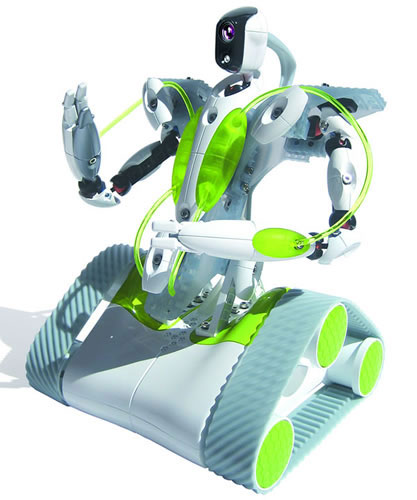
\includegraphics[scale=0.4]{images/spykee}
\caption{Il robot Spykee utilizzato nel progetto}
\end{figure}

\subsection*{Aggiunte hardware}
A partire da quanto già realizzato nei precedenti progetti, Spykee è stato dotato di ulteriori sensori che lo rendono adatto all'utilizzo all'interno del gioco. Tutti i componenti hardware aggiunti al robot sono controllati da un microcontrollore. A questo scopo è stata utilizzata una scheda STM32F4 Discovery Board della ST, dotata di un processore ARM Cortex M4, scelta per le sue caratteristiche: in particolare il grande numero di porte (GPIO, timer, seriali) utilizzabili.

Il firmware realizzato per controllare i vari dispositivi è stato sviluppato utilizzando il sistema operativo ChibiOS/RT\cite{chibios}. L'utilizzo di un sistema operativo per microcontrollori permette di utilizzare concetti quali thread e mutex, nonché di astrarre l'hardware sottostante, consentendo quindi una certa modularità (isolando ogni funzione in un thread indipendente) e quindi un rapido sviluppo del firmware.

La Discovery Board comunica con l'unità di elaborazione tramite un collegamento wireless di tipo Zigbee (utilizzando un modulo XBee della Digi). Il protocollo Zigbee è caratterizzato da una bassa velocità di trasmissione (comunque ampiamente sufficiente per gli scopi del progetto), ma da una buona facilità di utilizzo, specialmente in ambito embedded: viene infatti utilizzato come un collegamento seriale punto-punto tra microcontrollore e computer.

%TODO sistemare!
Le varie schede elettroniche sono state raccolte in una apposita scatola, e sono alimentate dal pacco batteria di Spykee tramite un regolatore di tensione, che permette di ridurre la tensione proveniente dalla batteria (circa $9$ V) a quella di $5$ V. Un apposito interruttore, posto a valle dell'interruttore di alimentazione di Spykee, permette di spegnere o accendere le aggiunte hardware.

\paragraph{Sonar e led} Per rilevare, e quindi evitare, eventuali ostacoli incontrati durante il movimento del robot, sono stati montati quattro sonar MaxSonar\textregistered-EZ della MaxBotix, uno per ognuno dei punti cardinali (nord, sud, ovest, est). L'aggiunta di questo tipo di dispositivi è necessaria in quanto il robot non è progettato per muoversi autonomamente, ma soltanto per ricevere comandi impartiti manualmente. 

Inoltre, Spykee è stato dotato di due strisce di LED (quattro LED gialli, quattro rossi e uno verde) che permettono di mostrare alcune informazioni relative allo stato del robot e/o del gioco nel complesso.
\begin{nota}
Sul robot sono anche presenti due led a infrarossi, che venivano utilizzati insieme a un controller Wiimote in precedenti progetti, ma che non sono di interesse per questo gioco. Le altre aggiunte hardware verranno descritte nei paragrafi successivi, essendo strettamente collegate ad altri componenti del gioco.
\end{nota}

%TODO bisogna spiegare l'interfaccia del firmware? (comandi che riceve, pinout, ...)

\section{Ostacoli attivi}
%TODO questa roba è tutta da sistemare!!!
Un problema che si è posto riguarda l'implementazione delle \emph{trappole}, gli ostacoli che modificano il comportamento del robot.

Poiché nel gioco viene già utilizzata una telecamera per poter riconoscere alcuni oggetti, inizialmente si è pensato di implementare anche le trappole utilizzando meccanismi di visione artificiale. In particolare, sono stati presi in considerazione vari tipi di marker bidimensionali, in particolare i ``Data Matrix'' e i tag della libreria ``ARToolkitPlus''\footnote{A differenza dei codici Data Matrix, che sono pensati per contenere informazioni arbitrarie, ad esempio URL oppure informazioni di spedizione, i tag ARToolkitPlus codificano solo un id, e sono pensati per applicazioni di identificazione, localizzazione, \dots (anche in presenza di distorsioni nell'immagine o altre condizioni non ottimali).}. Purtroppo, questi meccanismi hanno dato scarsi risultati in termini di velocità oppure di qualità del riconoscimento. I difetti riscontrati sono, ad esempio, un'enorme dipendenza dalle condizioni di luce, scarsi risultati in movimento, dovuti anche alla lentezza degli algoritmi (specialmente nel caso dei Data Matrix), e alle pessime condizioni delle immagini catturate. Per questi motivi, le soluzioni basate sul riconoscimento di tag mediante visione sono state scartate.

Una soluzione che ha fornito prestazioni migliori, e che è stata adottata per l'implementazione del gioco, è l'uso di tag RFID passivi a 125 KHz, che tuttavia richiede l'aggiunta di ulteriore hardware. I tag vengono correttamente riconosciuti quando il robot passa sopra di essi, con un margine di errore accettabile. Inoltre, il loro formato (tessere di plastica della dimensione di una carta di credito) li rende abbastanza comodi per l'utilizzo da parte del giocatore. Per la lettura dei tag, è stato montato sul robot un lettore (l'ID-12 della ID-Innovations), che trasmette i dati mediante un collegamento seriale a 9600 bps alla scheda di controllo presente sul robot. Una limitazione di questo specifico modello di lettore è la presenza di un'antenna interna, che ne limita pesantemente il posizionamento.

\section{Torri e fabbriche}
Le torri e le fabbriche sono costituite semplicemente da cilindri di cartoncino di colori differenti, di dimensione tali da poter essere rilevati ed abbattuti dal robot. In particolare, si è utilizzato un cilindro di colore rosso per la torre, e tre cilindri più piccoli di colore giallo per le fabbriche. 

La base dei cilindri contiene un interruttore, che risulta chiuso quando il cilindro è appoggiato a terra, e viene aperto all'abbattimento della torre. L'apertura dell'interruttore attiva un trasmettitore (del tipo di quelli utilizzati per comandare i cancelli elettrici) che invia un segnale radio a un ricevitore posto sul robot, e quindi segnala all'unità di elaborazione l'abbattimento di una torre o di una fabbrica.

Il ricevitore montato sul robot è il RX-4M-HCS prodotto dall'Aurel, ed è dotato di quattro canali separati con uscita open-drain (corrispondenti ai quattro pulsanti presenti sui corrispondenti trasmettitori, sempre della stessa marca). Pertanto, si sono impostati i relativi ingressi del microcontrollore come ingressi pull-up. Le uscite del ricevitore possono essere impostate, durante l'associazione con i trasmettitori, sia in modalità monostabile (ossia sono attive quando l'interruttore è chiuso) che in modalità bistabile (cambiano stato alla pressione dell'interruttore). Per la nostra applicazione si è scelto di utilizzare la modalità monostabile.  %TODO quest'ultimo paragrafo è da rivedere!
\chapter{Architettura software}
\label{cap:architetturasw}

Per semplificare l'implementazione e agevolare il riuso del codice esistente, il software è stato realizzato utilizzando ROS (Robot Operating System) \cite{rosweb}. Si tratta di un middleware pensato per applicazioni robotiche costituite da un elevato numero di moduli, relativamente indipendenti, che interagiscono tra loro.

Un sistema realizzato con ROS è suddiviso in un certo numero di \emph{nodi}, ovvero semplici processi\footnote{attualmente ROS supporta C++ e Python} indipendenti, che vengono eseguiti in parallelo e svolgono ciascuno una funzione elementare. Per migliorare l'organizzazione (e la distribuzione) del codice sorgente, i nodi possono poi essere raggruppati in \emph{package}. A loro volta, un gruppo di package può formare uno \emph{stack}. ROS mette a disposizione due differenti tecniche con cui i nodi possono comunicare tra loro:
\begin{itemize}
 \item un paradigma ``publish-subscribe'': i nodi pubblicano (\emph{publish}) messaggi su un certo argomento (\emph{topic}). I destinatari della comunicazione sono i nodi iscritti (\emph{subscribe}) a quel topic.
 \item l'invocazione di \emph{servizi} esposti da altri nodi, con la possibilità di ricevere una risposta, secondo una semantica simile a quella di una chiamata di procedura remota (RPC)
\end{itemize}

Oltre a funzionare come middleware di comunicazione interprocesso, ROS mette a disposizione alcuni programmi grafici e testuali, e funzioni di libreria che forniscono funzioni utili allo sviluppo di applicazioni robotiche.

Il sistema da noi realizzato risulta quindi composto da vari nodi. Ciascuno di essi è contenuto in un package omonimo all'interno della directory principale del progetto. In figura \ref{fig:schemanodi} è rappresentata l'architettura generale del sistema: in particolare i vari nodi e le dipendenze dalle librerie esterne a ROS. Le frecce rappresentano la comunicazione tra nodi (messaggi scambiati e servizi invocati) e i canali di comunicazione tra il software presente sull'unità di elaborazione e il robot.

\begin{figure}[h]
\resizebox{\linewidth}{!}{%
\begin{tikzpicture}[node distance=1cm, auto]
\tikzset{
   mynode/.style={rectangle,rounded corners,draw=black, top color=white, bottom color=white!50, thick, inner sep=1em, minimum size=3em, text centered},
   mynode2/.style={rectangle,rounded corners,draw=black, top color=white, bottom color=white!50, dashed, inner sep=1em, minimum size=1em, text centered},
}  
\node[mynode] (spykee) {\textbf{SpyKee}}; 
\node[mynode, below=4cm of spykee] (echoes) {\textbf{Echoes}}; 
\node[mynode, right=5cm of spykee] (vision) {\textbf{Vision}}; 
\node[mynode, below right=3cm of vision] (isaac) {\textbf{IsAac}}; 
\node[mynode2, below=1cm of isaac] (brian) {\emph{Mr. BRIAN}}; 
\node[mynode2, below left= 2cm of spykee] (robot) {\emph{Robot}}; 
\node[mynode2, above=1cm of vision] (opencv) {\emph{OpenCV + Blob Growing Algorithm}}; 
 
\draw[->, >=latex', shorten >=2pt, shorten <=2pt, bend left=10, thick] 
     (spykee.east) to node[auto, swap] {\ttfamily{spykee\_camera}}(vision.west); 

\draw[->, >=latex', shorten >=2pt, shorten <=2pt, bend left=10, thick] 
     (isaac.west) to node[auto, swap] {\ttfamily{spykee\_motion}}(spykee.south); 

\draw[->, >=latex', shorten >=2pt, shorten <=2pt, bend right=20, thick] 
     (echoes.east) to node[auto,swap] {\ttfamily{\begin{tabular}{c}
	 sonar\_data \\
     rfid\_data \\
     towers\_data
  \end{tabular}
}}(isaac.west); 
     
\draw[->, >=latex', shorten >=2pt, shorten <=2pt, bend right=10, thick, dashed] 
     (isaac.west) to node[auto, swap] {{\ttfamily{led\_data}} (servizio)}(echoes.east); 

\draw[->, >=latex', shorten >=2pt, shorten <=2pt, bend left=30, thick] 
     (vision.east) to node[auto, swap] {{\ttfamily{vision\_results}}}(isaac.north); 

\draw[<->, >=latex', shorten >=2pt, shorten <=2pt, bend left=0, thin, dashed] 
     (isaac.south) to node[auto, swap] {}(brian.north); 

\draw[<->, >=latex', shorten >=2pt, shorten <=2pt, bend left=0, thin, dashed] 
     (vision.north) to node[auto, swap] {}(opencv.south); 

\draw[<->, >=latex', shorten >=2pt, shorten <=2pt, bend left=7, thin, dashed] 
     (robot.north) to node[auto, swap] {Wi-fi}(spykee.west); 

\draw[<->, >=latex', shorten >=2pt, shorten <=2pt, bend right=7, thin, dashed] 
     (robot.south) to node[auto, swap] {Zigbee}(echoes.west); 

% The swap command corrects the placement of the text.

\end{tikzpicture} 
} 
\medskip

\caption{Struttura generale del sistema} 
\label{fig:schemanodi}
\end{figure}

\section{SpyKee}
\emph{SpyKee} si occupa di interfacciare l'unità di elaborazione con le funzioni del robot che comunicano via Wi-Fi: permette di fornire i comandi ai cingoli e di ricevere le immagini catturate dalla telecamera. Questo nodo è frutto dell'adattamento a ROS di una libreria realizzata nei precedenti progetti, e ottenuta analizzando con un software di cattura dei pacchetti di rete la comunicazione tra il robot e il software di controllo per Microsoft Windows fornito dalla Meccano.

SpyKee pubblica messaggi di tipo \verb|std_msgs::CompressedImage| sull'argomento \verb|spykee_camera|, che contengono le immagini ricevute dalla telecamera compresse in formato JPEG. Inoltre sottoscrive messaggi di tipo \verb|SpyKee::Motion| sull'argomento \verb|spykee_motion|, contenenti i comandi da inviare ai cingoli. Tali comandi sono costituiti da due interi compresi tra $-90$ e $90$, che rappresentano la velocità tangenziale e angolare del robot, e vengono convertiti dal nodo nei corrispondenti comandi al cingolo destro e sinistro.

\section{Echoes}
\emph{Echoes} comunica via Zigbee con l'hardware aggiunto a posteriori al robot: sonar, led, lettore RFID, e ricevitori dei comandi inviati dagli interruttori posti sulle torri e sulle fabbriche.

Il nodo riceve i dati dalla porta seriale\footnote{di default viene utilizzato il device \texttt{/dev/ttyUSB0}, altrimenti il percorso deve essere fornito da riga di comando come primo argomento}, analizza le stringhe ricevute, e pubblica i messaggi contenenti i dati rilevati:
\begin{itemize}
	\item i messaggi di tipo \verb|Echoes::Sonar| sull'argomento \verb|sonar_data| contengono i dati ricevuti dai sonar (valori delle distanze dei quattro sonar montati sul robot, espresse in millimetri).
	\item i messaggi di tipo \verb|Echoes::Rfid| sull'argomento \verb|rfid_data| contengono semplicemente una stringa identificativa del tag RFID rilevato
	\item i messaggi di tipo \verb|Echoes::Tower| sull'argomento \verb|towers_data| contengono un intero che corrisponde all'id della torre (o della fabbrica) abbattuta
\end{itemize}
Inoltre, il nodo espone un servizio di tipo \verb|Echoes::Led|, \verb|led_data|, che permette di controllare l'accensione dei led, e un altro servizio che consente di spegnere tutti i led (\verb|resetLed_data|). I led possono essere impostati nello stato di acceso, spento o lampeggiante. In particolare, per i led gialli e i led rossi, lo stato lampeggiante viene definito a livello dell'intero gruppo di led.

A causa dell'alto rumore presente nei valori provenienti dai sonar, il valore $x_k$ che viene pubblicato sul topic \verb|sonar_data| è filtrato attraverso un filtro a media mobile esponenziale. Questo significa che il dato pubblicato all'arrivo del $k$-esimo campione $x_{cur}$ registrato dal sonar è dato da
  \[ x_k = \alpha x_{cur} + (1 - \alpha) x_{k-1} \]
dove $\alpha = 0.3$, valore sufficientemente basso da ridurre il rumore ad alta frequenza presente nel segnale, ma comunque abbastanza alto da rendere l'aggiornamento dei valori reattivo, e riuscire ad evitare efficacemente gli ostacoli.

\section{Vision: identificazione degli oggetti}

\emph{Vision} si occupa di analizzare le immagini provenienti dalla telecamera di Spykee, per rilevare la presenza di una torre o di una fabbrica. 

Il nodo riceve da \emph{SpyKee} i messaggi contenenti le immagini e, analizzata l'immagine, pubblica un messaggio di tipo \verb|Vision::Results| sull'argomento \verb|vision_results|. Questo messaggio contiene i dati riguardanti gli oggetti trovati: la posizione rispetto al centro dell'immagine, una stima della distanza in centimetri, e l'altezza e la larghezza del blob in pixel.

Il cuore del nodo è un algoritmo, già utilizzato nel progetto \cite{docmandelli}, che si occupa di identificare all'interno dell'immagine dei blob sufficientemente uniformi e di colore ``simile'' a quello degli oggetti che si stanno cercando. L'analisi viene effettuata basandosi su un algoritmo di tipo KNN, che necessita di una prima fase di addestramento. Al termine di questa fase, viene generato un classificatore (contenuto in un file \verb|.kcc|), tramite il quale l'algoritmo è in grado di associare ad ogni pixel dell'immagine una classe di identificazione. Le classi riguardano i pixel di colore simile a quello di una torre (classe \verb|R|), oppure di una fabbrica (classe \verb|G|). Una volta effettuata la classificazione dei pixel dell'immagine, l'algoritmo per rileva all'interno dell'immagine i blob di interesse, e quindi stabilisce se è presente una torre o una fabbrica.

Il classificatore viene generato a partire da un file che contiene semplicemente un elenco di valori \verb|BGR| di pixel che si considerano del colore cercato. Per generare questo file è possibile utilizzare il nodo \emph{LittleEndian}: questo nodo carica le immagini da file oppure le riceve direttamente da \emph{SpyKee}, e consente di evidenziare nell'immagine le aree che corrispondono agli oggetti cercati. Alla fine, LittleEndian genera un file \verb|.dts| che contiene l'insieme dei valori. Per generare il classificatore, è sufficiente lanciare una volta \emph{Vision} indicando come parametro \verb|-L <filename.dts>|.

%TODO filtraggio etc?

\begin{nota}
È necessario prestare particolare attenzione nel training del classificatore, in quanto è una fase critica per il corretto funzionamento del gioco e il corretto riconoscimento degli oggetti.
\end{nota}

\section{RoboTower\_Game: la logica di gioco}
\begin{figure}
\centering
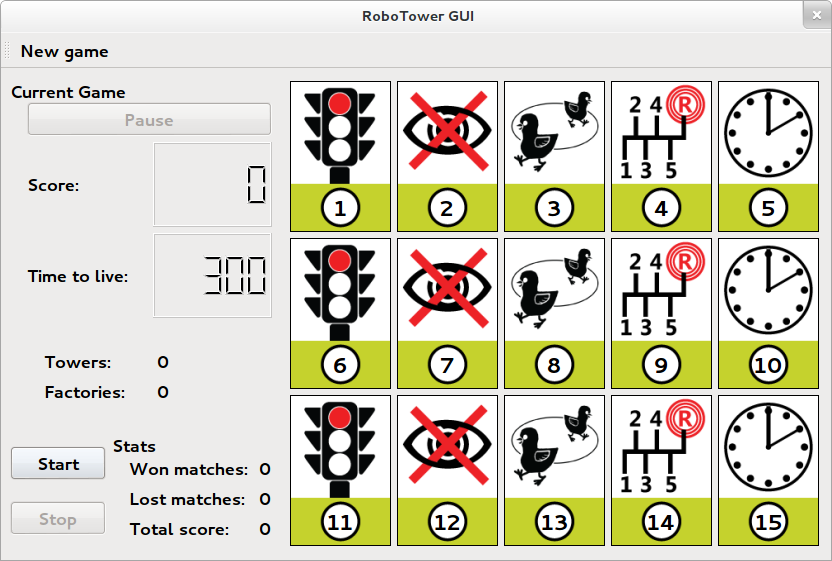
\includegraphics[scale=0.43]{images/rtgame}
\caption{Schermata principale dell'interfaccia di controllo del gioco}
\end{figure}

\emph{RoboTower\_Game} gestisce la logica ad ``alto livello'' del gioco e la comunicazione con l'utente tramite un'apposita interfaccia grafica, realizzata con le librerie Qt \cite{qtweb}. Si occupa di avviare e arrestare le partite, gestire lo stato del gioco, contare i punti, e tenere alcune semplici statistiche. Il nodo interagisce con gli altri processi:
\begin{itemize}
\item avviando e fermando il comportamento di basso livello del robot, a seconda dello stato corrente del gioco (pubblicando messaggi di tipo \verb|std_msgs::Bool| sull'argomento \verb|isaac_enable|)
\item ricevendo da \verb|Echoes| gli ID dei tag RFID letti e le informazioni riguardanti eventuali abbattimenti di torri o fabbriche
\item pubblicando messaggi di tipo \verb|std_msgs::String| sull'argomento \verb|rfid_actions| relativi alle azioni speciali che devono essere eseguite dal robot, come spiegato nel seguito
\item invocando i servizi relativi all'accensione e allo spegnimento dei led relativi al punteggio
\end{itemize}

\begin{figure}[h]
{
\lstset{
  language=XML,
  morekeywords={encoding, robotower, config, time, points, goals, rfid, action, tag}}
\begin{lstlisting}
<robotower>
	<config>
		<time timetolive="300" setuptime="30" />
		<points tower="100" factory="30" />
		<goals towerid="4" factories="3" />
		<recharge tower="3" factory="2"/>
	</config>

	<rfid>
		<action name="lock_all">
			<tag id="4400F56CD1" num="1" />
			<tag id="4400F59195" num="2" />
			<tag id="4400F58B6D" num="3" />
		</action>
      
		<action name="disable_vision">
			<tag id="4400BDB1D9" num="4" />
			<tag id="4400BDC253" num="5" />
			<tag id="4B00DA3279" num="6" />
		</action>
	</rfid>
</robotower>
\end{lstlisting}
}
\caption{Il file di configurazione}
\label{fig:configfile}
\end{figure}

La maggior parte delle impostazioni di RoboTower\_Game possono essere configurate modificando il file \verb|robotower.xml|, che si trova nella directory \verb|RoboTower_Game|. Un esempio di file di configurazione corretto è riportato in figura \ref{fig:configfile}\footnote{per semplicità sono stati omessi alcuni tag RFID e le relative azioni}. Nel file è possibile specificare:
\begin{itemize}
\item I tempi del gioco (tag \lstinline|<time>|): l'attributo \lstinline|timetolive| permette di modificare la durata massima di un round del gioco, mentre l'attributo \lstinline|setuptime| controlla il tempo che deve trascorrere dall'inizio della partita (pressione del pulsante ``start'') e l'inizio del movimento del robot
\item I parametri con cui viene calcolato il punteggio (tag \lstinline|<points>|): durante la partita, ogni secondo viene aggiunto un certo numero di punti per ogni torre e fabbrica che non sono stati ancora distrutti, definiti dagli attributi \lstinline|tower| e \lstinline|factory|
\item I parametri relativi a torre e fabbriche (tag \lstinline|<goals>|): in particolare, il numero di fabbriche (\lstinline|factories|) e l'id dell'obiettivo che dev'essere considerato come torre (\lstinline|towerid|)
\end{itemize}
Il nodo si occupa inoltre di gestire i comportamenti ``speciali'' del robot, collegati alle trappole (tag RFID). Per ogni trappola, è necessario specificare, all'interno del blocco \lstinline|<action>| relativo all'azione associata, l'id e un numero (univoco) che viene utilizzato per identificarlo nell'interfaccia grafica. Le azioni che possono essere specificate (parametri \lstinline|name|) sono:
\begin{itemize}
\item \lstinline|lock_all|: blocca per 5 secondi i motori del robot
\item \lstinline|force_rotate|: costringe per 5 secondi il robot a ruotare su se stesso, inibendo i comandi diretti a uno dei due cingoli
\item \lstinline|disable_vision|: disabilita la visione del robot per 5 secondi
\item \lstinline|go_back|: blocca per 5 secondi l'avanzamento del robot, costringendolo a tornare indietro
\item \lstinline|modify_time|: modifica casualmente il tempo rimanente alla fine del round (sia in positivo che in negativo)
\end{itemize}
Una volta che viene letto un tag, questo viene disabilitato. I tag possono essere ricaricati, uno alla volta, dopo un periodo di tempo che dipende dal numero di fabbriche residue sul campo di gioco.

\section{IsAac: il comportamento del robot}
\emph{IsAac} si occupa di controllare il comportamento di ``basso livello'' del robot durante il gioco. In base ai dati provenienti dai sensori, gestisce il comportamento del robot, impostando i set-point per i cingoli e controllando l'accensione di alcuni led.

Il nodo riceve i messaggi pubblicati da \emph{Echoes} e \emph{Vision}, e invia comandi a \emph{SpyKee} (messaggi \verb|Spykee::Motion| sull'argomento \verb|spykee_motion|) riguardanti il controllo dei cingoli. Inoltre invoca il servizio \verb|led_data| esposto da Echoes per il controllo dei led gialli e del led verde posti sul robot. I led gialli lampeggiano quando \emph{IsAac} è attivo, sono spenti quando non è attivo, e rimangono accesi quando il robot è bloccato in una trappola. Il led verde lampeggia quando viene rilevata una torre o una fabbrica, altrimenti è spento.

\emph{IsAac} riceve da \emph{RoboTower\_Game} i comandi di attivazione e disattivazione, e le informazioni riguardanti il blocco del robot in una trappola (quando l'azione a cui è associata richiede la modifica dei dati provenienti dai sensori oppure dei comandi diretti agli attuatori, in caso contrario l'azione è implementata direttamente in \emph{RoboTower\_Game}).

Per l'implementazione di questo nodo, è stata sfruttata la libreria Mr. Brian, sviluppata dal Politecnico di Milano nel contesto di di MRT (Modular Robotic Toolkit) \cite{mrt}. Questa libreria consente di definire il comportamento da applicare al robot come un insieme di regole scritte in \emph{logica fuzzy}, utilizzando anche predicati che risultano dalla fuzzyficazione degli ingressi. La configurazione di Brian è basata su un insieme di file di testo: in questo modo è possibile modificare totalmente i comportamenti senza bisogno di ricompilare il codice sorgente. I file di configurazione, presenti nella cartella \verb|IsAac/config|, sono:
\begin{itemize}
\item \verb|behaviour.txt| contiene l'elenco, suddiviso per livelli, dei comportamenti (regole) che sono stati definiti. Ogni comportamento, costituito da un insieme di regole fuzzy, è contenuto in un file \verb|.rul|
\item \verb|ctof.txt| associa ad ogni dato crisp in ingresso un'insieme fuzzy, che verrà utilizzato per la fase di fuzzyficazione. Gli insiemi fuzzy sono definiti nel file \verb|shape_ctof.txt|.
\item \verb|s_ftoc.txt| definisce i valori in uscita da Brian, associandoli agli insiemi fuzzy da utilizzare per la defuzzyficazione. Gli insiemi sono definiti nel file \verb|s_shape.txt|
\item \verb|Predicate.ini| definisce i predicati fuzzy sulla base di variabili fuzzy e/o di altri predicati
\item \verb|Cando.ini| definisce le condizioni di attivazione per un determinato comportamento (le condizioni necessarie per cui eseguire quel comportamento sia sensato)
\item \verb|Want.ini| definisce le condizioni per cui è opportuno attivare un determinato comportamento
\end{itemize}
La suddivisione in livelli nel file \verb|behaviour.txt| permette di utilizzare come ingresso dati in uscita dai livelli precedenti, ed eventualmente cancellare anche le uscite impostate dai livelli precedenti. Nelle regole, infatti, è possibile utilizzare anche i predicati che sono stati definiti nel file \verb|PredicateActions.ini|. In questo file è possibile far riferimento ai dati in uscita dai livelli precedenti a quello corrente, utilizzando etichette della forma
\begin{center}\verb|Proposed<nome del dato in uscita>|\end{center}
dopo averle associate ad opportuni insiemi fuzzy nel file \verb|ctof.txt|. La suddivisione in livelli permette di rendere maggiormente modulari le regole fuzzy. All'interno del manuale di MRT \cite{mrtmanual} è presente la descrizione completa del funzionamento di Mr. Brian e della sintassi dei file di configurazione.

I comportamenti che sono stati implementati riguardano:
\begin{itemize}
 \item Cercare casualmente la torre o le fabbriche (Search.rul)
 \item Raggiungere la torre o la fabbrica, una volta che è stata trovata (GoToTower.rul e GoToFactory.rul)
 \item Evitare gli ostacoli (AvoidObstacle.rul, KeepDistance.rul, GoBack.rul)
 \item Distruggere la torre o una fabbrica (Destroy.rul)
\end{itemize}
\chapter{Conclusioni}
%\markboth{Introduzione}{Introduzione}
\label{cap:conclusioni}

\begin{figure}
\centering
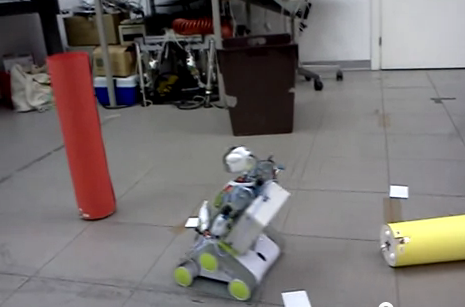
\includegraphics[scale=0.3]{images/attaccotorre}
\caption{Spykee va all'attacco della torre}
\end{figure}

Dalle prove che abbiamo effettuato, \emph{RoboTower} risulta giocabile e coinvolgente per il giocatore. Variando il numero e la dimensione degli ostacoli fissi, oppure agendo sui parametri di configurazione, quali la durata del singolo round oppure il tempo di ricarica delle carte, è possibile rendere il gioco più o meno difficile, e quindi adattarlo al giocatore. Agendo sulla dimensione del campo di gioco, invece, è possibile porre maggiormente l'accento sull'aspetto strategico del gioco (posizionamento corretto degli ostacoli, delle torri e delle fabbriche all'inizio del gioco), oppure su quello dinamico (posizionamento delle trappole durante l'avanzata del robot). Perché il gioco funzioni correttamente, comunque, il campo di gioco, deve avere una dimensione abbastanza piccola (ad esempio, un quadrato di lato $4$ m).

Le maggiori problematiche relative all'implementazione del gioco riguardano alcuni limiti degli strumenti a disposizione, in particolare del sistema di visione e del controllo del movimento. Per quanto riguarda la visione, il funzionamento degli algoritmi è fortemente inficiato dalla qualità dell'immagine proveniente dalla telecamera. Le immagini, infatti, a causa della forte compressione JPEG cui sono sottoposte, hanno visibili artefatti che influenzano negativamente il riconoscimento dei blob colorati. Purtroppo, essendo la compressione effettuata a bordo del robot, non è possibile ridurre la compressione. Altri problemi della visione sono legati alla forte dipendenza alle condizioni di luminosità dell'algoritmo di visione utilizzato, che rende necessario effettuare più volte il training del classificatore, a seconda delle condizioni di luce.

Per quanto riguarda il controllo del movimento, l'imprecisione dei comandi ricevuti dal robot e la strategia di controllo attuata (ad anello aperto) rendono impossibile controllarne l'effetto sull'attuale hardware. Questo provoca dipendenza della risposta del robot ai comandi da molteplici fattori, come la carica della batteria e la superficie su cui si muove. I frequenti ritardi nella trasmissione dei comandi, e il fatto che questi vengano eseguiti in coda, rendono difficile far agire il robot in maniera istantanea. A causa della mancanza di opportuni sensori, risulta impossibile creare una mappa dell'ambiente, o più semplicemente mantenere informazioni riguardo le posizioni di alcuni elementi rispetto al robot: questo non permette di attuare strategie complesse, che tengano conto della posizione degli oggetti già visti, e di pianificare in maniera adeguata l'aggiramento degli ostacoli.

I maggiori successi nell'implementazione del robot provengono dallo sfruttamento della logica fuzzy e da MrBrian, che ben si adattano a situazioni poco definite, come lo sono i dati che vengono estratti dai sensori del robot. Tramite regole fuzzy, si è riusciti a implementare un comportamento che risponde abbastanza bene agli stimoli dell'ambiente, rendendo il robot in grado di evitare ostacoli in maniera abbastanza soddisfacente e di puntare gli obiettivi seguendo delle traiettorie abbastanza pulite e razionali, nonostante il controllo impreciso dei motori.

Altri ottimi risultati sono arrivati grazie al middleware ROS, che ha consentito un forte disaccoppiamento delle parti del sistema, favorendo la riusabilità dei componenti. È facile quindi re-implementare parte del codice per portare RoboTower su altri robot. Inoltre, fornisce  moltissimi tool grafici e da linea di comando per semplificare il debug e il design delle applicazioni. 

%TODO accennare al riconoscimento giocatore x evitare che si metta davanti alla torre???

\section*{Ringraziamenti}

Ringraziamo Davide Perego per averci fornito le immagini, sia per gran parte delle carte, sia per il logo dell'interfaccia grafica del gioco RoboTower.

Un grosso ringraziamento va inoltre a tutto lo "staff" dell'AIRlab per il loro grandissimo supporto durante tutto lo svolgimento del progetto, in particolare il prof. Bonarini, Davide Rizzi e Martino Migliavacca: il loro aiuto ci è stato fondamentale!

% Appendici for now don't needed!
\appendix
\chapter{Installazione del software}
%\markboth{Introduzione}{Introduzione}
\label{cap:installazione}

Le istruzioni per la compilazione e l'utilizzo del software si riferiscono a un sistema Linux, e sono state testate con le distribuzioni Debian e Ubuntu 12.04.

\section{Compilare il sorgente}

Qui va l'elenco delle dipendenze e le istruzioni per compilare ed eseguire il tutto più
le istruzioni per eseguire il gioco

serve ROS, poi ???

\section{Avvio del gioco}

%TODO qui vanno le istruzioni su come utilizzare il sw
Per avviare ROS e i nodi che controllano il robot, è sufficiente il comando
\begin{verbatim}
roslaunch spykee.launch
\end{verbatim}
dalla cartella del progetto. Per avviare il gioco, avviare il programma \verb|isaac| presente nella directory \verb|IsAac/bin|. Per fermare il robot, è sufficiente chiudere quest'ultimo programma.

\section{Firmware del microcontrollore}

Il firmware è stato realizzato per la scheda (Evaluation Board) STM32F4 Discovery della ST. Nelle istruzioni che seguono, verrà utilizzato il programmatore integrato sulla scheda (ST-Link v2).

\subsection*{Prerequisiti}
\begin{enumerate}
\item Installare una toolchain GNU per ARM, ad esempio CodeSourceryLite, ed aggiungerla nel PATH dell’utente. Nel seguito si suppone che i binari del crosscompilatore gcc per ARM e del debugger siano disponibili nel PATH e raggiungibili rispettivamente dai comandi \verb|arm-none-eabi-gcc| e \verb|arm-none-eabi-gdb|. Se i comandi sono diversi (o non sono presenti nel PATH), è necessario cambiare di conseguenza il \verb|Makefile| del progetto.

\item Installare OpenOCD, scaricabile da \url{http://openocd.sourceforge.net}. Potrebbe essere necessario installare alcune dipendenze, elencate comunque nella documentazione del programma.

\textbf{Nota } Al momento della scrittura del presente manuale (luglio 2012), il programmatore ST-Link v2 è ufficialmente supportato solo sulla piattaforma Windows. Tuttavia, è presente un supporto sperimentale in OpenOCD: per poterlo utilizzare, è necessario scaricare e compilare la release di sviluppo dal repository git di sviluppo (\url{http://sourceforge.net/scm/?type=git&group_id=274635}). Una volta scaricati i sorgenti, è sufficiente compilarli tramite i seguenti comandi  (dalla cartella in cui si è clonato il repository):
\begin{verbatim}
   $ ./configure --enable-maintainer-mode --enable-stlink
   $ make
   # make install
\end{verbatim}
L’ultimo comando serve per installare OpenOCD nelle cartelle di sistema, e dev'essere eseguito con i privilegi di root.

\item Scaricare i sorgenti di ChibiOS da \url{http://chibios.org}. Una volta scaricato e decompresso l'archivio, aprire il \verb|Makefile| presente nella cartella FirmwareSpykee e modificare la riga
\begin{verbatim}
   CHIBIOS=/home/stm32/Workspace/libs/ChibiOS
\end{verbatim}
inserendo il percorso corretto. Il firmware è stato testato con la versione 2.4.1 di ChibiOS.
\end{enumerate}

\subsection*{Compilazione ed installazione}

\paragraph{Compilazione} Posizionarsi nella cartella FirmwareSpykee e dare il comando
\begin{verbatim}
   $ make
\end{verbatim}
Se la compilazione ha successo, viene prodotto il file \verb|ch.elf| nella sottocartella \verb|build|.

\paragraph{Installazione} Per caricare il firmware sulla scheda, è necessario prima di tutto collegare la scheda al computer e avviare OpenOCD con il comando
\begin{verbatim}
   $ openocd -f board/stm32f4discovery.cfg
\end{verbatim}
Quindi, mantenendo aperto OpenOCD, collegare il debugger gdb:
\begin{verbatim}
   $ arm-none-eabi-gdb ch.elf
   (gdb) target extended-remote localhost:3333
\end{verbatim}
dove \verb|ch.elf| è il percorso del firmware compilato che si vuole caricare sulla scheda. Una volta che \verb|gdb| è connesso ad OpenOCD, la seguente sequenza di comandi cancella il contenuto della memoria FLASH, carica il nuovo firmware, e quindi lo avvia:
\begin{verbatim}
   (gdb) monitor reset halt
   (gdb) monitor flash probe 0 
   (gdb) monitor stm32f2x mass_erase 0 
   (gdb) load 
   (gdb) monitor reset halt 
   (gdb) continue
\end{verbatim}

\textbf{Nota } A volte la scheda non viene riconosciuta da OpenOCD. Questo problema a volte viene risolto tenendo premuto il pulsante RESET sulla scheda mentre si avvia openOCD. Se anche così non funziona, è necessario cancellare il contenuto della memoria flash con l’utility ST Visual Programmer (disponibile solo per Windows).
%TODO non so se è il caso di mettere qui la corrispondenza pin <-> connessione o basta metterla nel README nella cartella FirmwareSpykee

\section{Collegamenti hardware}
Il file board.h permette di configurare le funzioni assegnate ai vari della Discovery Board presente nel robot. Attualmente, i pin presenti sulla scheda sono assegnati in questo modo:
\begin{itemize}
\item Collegamento con i sonar (timer): \verb|PA8| (nord), \verb|PB4| (sud), \verb|PA0| (ovest), \verb|PC6| (est)
\item Seriale per collegamento con lo XBee, bitrate 19200 bps: \verb|PA2| (TX) e \verb|PA3| (RX)
\item Ricevitore dei segnali inviati
	\begin{itemize}
	\item Dalle fabbriche: \verb|PD0|, \verb|PD1| e \verb|PD2|
	\item Dalla torre: \verb|PD3|
	\end{itemize}
\item Led presenti sul robot:
	\begin{itemize}
	\item Led rossi: \verb|PE7| (0), \verb|PE8| (1), \verb|PE9| (2), \verb|PE10| (3)
	\item Led gialli: \verb|PE11| (0), \verb|PE12| (1), \verb|PE13| (3), \verb|PE14| (4)
	\item Led verde: \verb|PE15|
	\item Led a infrarossi (sulle spalle del robot): \verb|PD11|
	\end{itemize}
\item Lettore RFID (collegamento seriale a 9600 bps): \verb|PB11| (RX)
\end{itemize}
% \include con i nomi dei capitoli

% --------------------------------------------------------------------------------------------------------------------
% Bibliografia - nothing for now!
\bibliographystyle{plain}
\begin{thebibliography}{9}

\bibitem{rosweb}
  ROS Wiki, \url{www.ros.org}

\bibitem{spykeeweb}
  Meccano, Spykee: the Spy Robot, \url{http://www.spykeeworld.com}

\bibitem{chibios}
  The ChibiOS/RT Project, \url{http://chibios.org}

\bibitem{qtweb}
	Qt - Cross-platform application and UI framework, \url{http://qt.nokia.com}

\bibitem{robowii}
  Progetto RoboWii, \url{http://airlab.elet.polimi.it/index.php/ROBOWII}

\bibitem{mrtmanual}
  MRT: Modular Robotics Toolkit, \url{http://airlab.elet.polimi.it/index.php/MRT}

\bibitem{mrt}
  A. Bonarini, M. Matteucci, M. Restelli, \emph{MRT: Robotics Off-the-Shelf with the Modular Robotic Toolkit},
  in D. Brugali (ed.), \emph{Software Engineering for Experimental Robotics}, STAR 30, Berlin, Springer-Verlag, 2007, 345-364

\bibitem{docmandelli}
  C. Mandelli, D. Zamponi, \emph{RoboWII 2.1: Implementazione di un gioco robotico}, \url{http://airlab.elet.polimi.it/images/1/1f/RoboWii_2.1-ZamponiMandelli.pdf}

\bibitem{brian}
  A. Bonarini, M. Matteucci, M. Restelli, \emph{Concepts and fuzzy models for behavior-based robotics}, International Journal of Approximate Reasoning \textbf{41} (2006), 110-127

\bibitem{st}
  Discovery kit for STM32 F4 series, \url{http://www.st.com/internet/evalboard/product/252419.jsp}

\bibitem{UbuntuDistro}
  Ubuntu, \url{http://www.ubuntu.com/download/desktop}

\bibitem{DebianDistro}
  Debian -- The universal Operating System, \url{http://www.debian.org}

\end{thebibliography}


% --------------------------------------------------------------------------------------------------------------------

\end{document}
